\documentclass[10pt]{extarticle}

\usepackage[margin=1.8cm]{geometry}
\usepackage{xcolor}
\usepackage{amsmath,amssymb}
\usepackage{tcolorbox}
\usepackage{enumitem}
\usepackage{graphicx}
\usepackage[
  colorlinks=true,
  linkcolor=blue!50!black,
  citecolor=green!35!black,
  urlcolor=blue!60!black
]{hyperref}

\renewcommand{\sectionautorefname}{Section}
\renewcommand{\subsectionautorefname}{Section}
\renewcommand{\figureautorefname}{Figure}
\renewcommand{\tableautorefname}{Table}
\renewcommand{\equationautorefname}{Equation}

\setlist[enumerate]{
  leftmargin=3.5em,
  itemsep=1pt,
  topsep=3pt,
  parsep=0pt,
  partopsep=0pt
}

\title{Tanaka Certificates}
% \author{}
\date{\today}

\tcbset{
  notebox/.style={
    boxrule=0.3pt,
    arc=0.5mm,
    left=2mm,
    right=2mm,
    top=1.5mm,
    bottom=1.5mm,
    fonttitle=\bfseries
  }
}

\newtcolorbox{setup}{
  notebox,
  title=Setup,
  colback=blue!2,
  colbacktitle=blue!12,
  colframe=blue!25!black,
  coltitle=blue!45!black
}

\newtcolorbox{hypothesis}{
  notebox,
  title=Hypothesis,
  colback=yellow!3,
  colbacktitle=yellow!18,
  colframe=yellow!45!black,
  coltitle=yellow!25!black
}

\newtcolorbox{fact}{
  notebox,
  title=Fact,
  colback=green!2,
  colbacktitle=green!12,
  colframe=green!25!black,
  coltitle=green!30!black
}

\begin{document}

\maketitle

\begin{abstract}
  In these notes, I am building up the intuition and theory behind supermartingale certificates, with relaxed assumptions on the certificate function $V$. In particular, it is explored what happens when $V$ is not twice continously-differentiable, but instead piecewise twice continuously-differentiable.
\end{abstract}

\section{Piecewise linear certificates in dimension one}

Consider the following setup:

\begin{setup}
Let:
\begin{enumerate}
    \item $dX_t = f(X_t) dt + g(X_t) dW_t$ be a one-dimensional SDE.
    \item $V(x)$ be a piecewise linear function such that $V(x) = a_i x + b_i$, where $x \in \left( x_i, x_{i+1} \right)$.
    \item $V(x)$ is continuous at breakpoints: $V(x_i^+)=V(x_i^-) = V(x_i)$
    \item as a consequence, $V'_{-}(x_i) = a_{i-1},$ $V'_{+}(x_i) = a_i$
\end{enumerate}

\end{setup}

Now we will consider what conditions on $V$ are sufficient to guarantee that $V(X_t)$ is a supermartingale.

\begin{hypothesis}
Does concavity of $V(x)$ (along with an interior / drift term condition) guarantee that $V(X_t)$ is a supermartingale?
\end{hypothesis}

To answer this, let's apply the Itô-Tanaka formula to $V(X_t)$:
\begin{align}
    V(X_t) = V(X_0) + &\int_0^t V'(X_s) f(X_s) ds \\
        + &\int_0^t V'(X_s) g(X_s) dW_s \\
        + \frac{1}{2} &\sum_{i=1}^{n-1} \left( V'_{+}(x_i) - V'_{-}(x_i) \right) L_t^{x_i}(X) \\
\end{align}

We will focus on these terms: 

\begin{enumerate}
  \item $D_t = \int_0^t V'(X_s) f(X_s) ds$, the drift term
  \item $M_t = \int_0^t V'(X_s) g(X_s) dW_s$, the diffusion term (stochastic integral)
  \item $K_t = \frac{1}{2} \sum_{i=1}^{n-1} \left( V'_{+}(x_i) - V'_{-}(x_i) \right) L_t^{x_i}(X)$, the kink term
\end{enumerate}

we need to prove that $D_t + M_t + K_t$ is a supermartingale.

Some natural assumptions, which are sufficient to guarantee that $V(X_t)$ is a supermartingale, are the following:
\begin{enumerate}
  \item $f(x) V'(x) \leq 0$ for all $x \in (x_i, x_{i+1})$. This is because of the following:
  
  \begin{fact}
  If $f(X) V'(X) \leq 0$, then the drift term $D_t$ is a supermartingale. \\
  \linebreak
  \textbf{Proof:} We want to prove $\mathbb{E}[D_t | \mathcal{F}_s] \leq D_s$ for $s \leq t$.
  \begin{align}
    \mathbb{E}[D_t | \mathcal{F}_s] &= \mathbb{E}\left[\int_0^t V'(X_u) f(X_u) du \Big| \mathcal{F}_s\right] \\
    &= \int_0^s V'(X_u) f(X_u) du + \mathbb{E}\left[\int_s^t V'(X_u) f(X_u) du \Big| \mathcal{F}_s\right] \\
    &\leq D_s + 0 = D_s
  \end{align}
  \end{fact}

  \item $M_t$ is a martingale. Assuming $V(x)$ has finitely many pieces
  (as is the case for a neural network with ReLU activation functions), it is enough
  to impose a square-integrability condition on $g(x)$\footnote{For example,
  $\mathbb{E}\!\left[\int_0^t g(X_s)^2\,ds\right]<\infty$.}
  
  \item $V'_{+}(x_i) - V'_{-}(x_i) \leq 0 \iff a_{i-1} \geq a_i$, i.e. the \textbf{concavity condition}. This is because of the following:
  \begin{fact}
    If $V'_{+}(x_i) - V'_{-}(x_i) \leq 0$ and $L_t^{x_i}(X) \geq 0$, then the kink term $K_t$ is a supermartingale. \\
    \linebreak
    \textbf{Proof:} We want to prove $\mathbb{E}[K_t | \mathcal{F}_s] \leq K_s$ for $s \leq t$.
    \begin{align}
      \mathbb{E}[K_t | \mathcal{F}_s] &= \mathbb{E}\left[\frac{1}{2} \sum_{i=1}^{n-1} \left( V'_{+}(x_i) - V'_{
-}(x_i) \right) L_t^{x_i}(X) \Big| \mathcal{F}_s\right] \\
      &= \frac{1}{2} \sum_{i=1}^{n-1} \left( V'_{+}(x_i) - V'_{-}(x_i) \right) \mathbb{E}\left[L_t^{x_i}(X) | \mathcal{F}_s\right] \\
      &\leq \frac{1}{2} \sum_{i=1}^{n-1} \left( V'_{+}(x_i) - V'_{-}(x_i) \right) L_s^{x_i}(X) = K_s
    \end{align}
    Note that the inequality follows from the fact that $L_t^{x_i}(X)$ is non-decreasing in $t$, hence $\mathbb{E}\left[L_t^{x_i}(X) | \mathcal{F}_s\right] \geq \mathbb{E}\left[L_s^{x_i}(X) | \mathcal{F}_s\right] = L_s^{x_i}(X)$.
  \end{fact}

\end{enumerate}

We will consider what happens in different practical cases to these terms, including: 
\begin{enumerate}
  \item A simple one-dimensional SDE with a piecewise linear certificate.
  \item A pendulum with a stochastic torque, and $X_t$ measuring the angle of the pendulum.
  \item A network $b$ black and $w$ white nodes, with given transition probabilities, and $X_t$ measuring the amount of mass in the white nodes. 
\end{enumerate}
to ensure our assumptions are reasonable.

\subsection{Proof of the supermartingale property}

First, let's note the following:

\begin{fact}
  The sum of a martingale and a supermartingale is a supermartingale. \\
  \linebreak
  \textbf{Proof}: By definition, given a martingale $M_t$ and a supermartingale $S_t$, for $r < t$ we have 
  $\mathbb{E}[M_t | \mathcal{F}_r] = M_r$ and 
  $\mathbb{E}[M_t | \mathcal{F}_r] \leq S_r$. Then, for $r < t$:
  \begin{align}
    \mathbb{E}[M_t + S_t | \mathcal{F}_r] &= \mathbb{E}[M_t | \mathcal{F}_r] + \mathbb{E}[S_t | \mathcal{F}_r] \\
    &= M_r + \mathbb{E}[S_t | \mathcal{F}_r] \\
    &\leq M_r + S_r = (M + S)_r
  \end{align}
\
hence $M_t + S_t$ is a supermartingale.

\end{fact}

The drift term $D_t$ is a supermartingale by assumption 1. The kink term $K_t$ is a supermartingale by assumption 3. The stochastic integral $M_t$ is a martingale by assumption 2. Therefore, the sum of these three terms is a supermartingale (as a consequence of the previous fact), and hence $V(X_t)$ is a supermartingale.

\section{Piecewise $\mathcal{C}^2$ certificates in dimension one}

The setup is pretty similiar, with the exception that $V$ is now piecewise $\mathcal{C}^2$ instead of piecewise linear. 

\begin{setup}
Let:
\begin{enumerate}
    \item $dX_t = f(X_t) dt + g(X_t) dW_t$ be a one-dimensional SDE.
    \item $V(x)$ be a piecewise $\mathcal{C}^2$ function such that $V(x) \in \mathcal{C}^2$, where $x \in \left( x_i, x_{i+1} \right)$.
    \item $V(x)$ is continuous at breakpoints: $V(x_i^+)=V(x_i^-) = V(x_i)$.
\end{enumerate}

\end{setup}

We will again consider what conditions on $V$ are sufficient to guarantee that $V(X_t)$ is a supermartingale. Again, the natural hypothesis is:

\begin{hypothesis}
Does concavity of $V(x)$ (along with an interior / drift term condition) guarantee that $V(X_t)$ is a supermartingale?
\end{hypothesis}

We apply the Itô-Tanaka formula to $V(X_t)$, and we get similiar terms, with the addition of
\begin{equation}
  C_t = \frac{1}{2} \int_{0}^{t} V''(X_s) g^2(X_s) ds
\end{equation}

Since the integral in the $C_t$ term is over the same intervals as the $D_t$ term, we can combine them to recover the generator / Lie derivative term:
\begin{equation}
  D_t + C_t = \int_{0}^{t} \left( V'(X_s) f(X_s) + \frac{1}{2} V''(X_s) g^2(X_s) \right) ds = \int_{0}^{t} \mathcal{L} V(X_s) ds
\end{equation}

The proof that $V(X_t)$ is a supermartingale is similiar to the piecewise linear case, but now we need to impose the condition:
\begin{equation}
  \mathcal{L} V(x) = V'(x) f(x) + \frac{1}{2} V''(x) g^2(x) \leq 0
\end{equation}

\newpage

\section{Studying piecewise certificates on concrete one-dimensional examples}

Some useful examples to study are given in Tables~\ref{tab:kink-examples}
and~\ref{tab:curvature-examples}.

\begin{table}[t]
\centering
\caption{Piecewise linear certificates examples.}
\label{tab:kink-examples}
\begin{tabular}{lllll}
\hline
SDE & $V(x)$ & $D_t$ & $M_t$ & $K_t$ \\
\hline
$dX_t=dW_t$
&
$-|x|$
&
$0$
&
$\displaystyle \int_0^t -\operatorname{sgn}(X_s)\,dW_s$
&
$\displaystyle -L_t^0(X)$
\\[1.1em]

% $dX_t=dW_t$
% &
% $|x|$
% &
% $0$
% &
% $\displaystyle \int_0^t \operatorname{sgn}(X_s)\,dW_s$
% &
% $\displaystyle L_t^0(X)$
% \\[1.1em]

$dX_t=-X_t\,dt$
&
$|x|$
&
$\displaystyle -\int_0^t |X_s|\,ds$
&
$0$
&
$0$
\\
\hline
\end{tabular}
\end{table}

\begin{table}[t]
\centering
\caption{Piecewise $\mathcal{C}^2$ certificates examples.}
\label{tab:curvature-examples}
\resizebox{\textwidth}{!}{%
\begin{tabular}{llllll}
\hline
SDE & $V(x)$ & $D_t$ & $M_t$ & $C_t$ & $K_t$ \\
\hline
$dX_t=-\lambda X_t\,dt+\sigma\,dW_t$
&
$x^2$
&
$\displaystyle -2\lambda \int_0^t X_s^2\,ds$
&
$\displaystyle \int_0^t 2\sigma X_s\,dW_s$
&
$\displaystyle \sigma^2 t$
&
$0$
\\[1.1em]

$dX_t=dt+\sqrt{2}\,dW_t$
&
$\displaystyle x-\frac{x^2}{2}$
&
$\displaystyle \int_0^t (1-X_s)\,ds$
&
$\displaystyle \int_0^t (1-X_s)\sqrt{2}\,dW_s$
&
$\displaystyle -t$
&
$0$
\\[1.1em]

$dX_t=dW_t$
&
$\displaystyle
\begin{cases}
-\frac12 x^2, & x<0,\\
-x, & x\ge 0
\end{cases}$
&
$0$
&
$\displaystyle \int_0^t V'(X_s)\,dW_s$
&
$\displaystyle -\frac12\int_0^t \mathbf 1_{\{X_s<0\}}\,ds$
&
$\displaystyle -\frac12 L_t^0(X)$
\\
\hline
\end{tabular}%
}
\end{table}

\subsection{Ornstein--Uhlenbeck process in three parameter regimes}

Consider the Ornstein--Uhlenbeck process
\[
  dX_t=-\lambda X_t\,dt+\sigma\,dW_t
\]
with the quadratic certificate $V(x)=x^2$. Its generator is
\[
  \mathcal LV(x)=-2\lambda x^2+\sigma^2
  =-2\lambda\left(x^2-\frac{\sigma^2}{2\lambda}\right).
\]
Consequently, if
\[
  r=\frac{\sigma}{\sqrt{2\lambda}},
\]
then the generator is negative for $|x|>r$, zero for $|x|=r$, and positive
for $|x|<r$. The decomposition is
\[
  X_t^2-X_0^2
  =\underbrace{-2\lambda\int_0^t X_s^2\,ds}_{D_t}
  +\underbrace{2\sigma\int_0^t X_s\,dW_s}_{M_t}
  +\underbrace{\sigma^2t}_{C_t},
\]
with $K_t=0$.

Figure~\ref{fig:ou-terms} fixes $\lambda=1$ and $X_0=1$, and uses
$r=0.5$, $r=1$, and $r=1.5$. These choices make the initial generator
negative, zero, and positive, respectively. Moreover,
\[
  \mathbb E[X_t^2]
  =r^2+(X_0^2-r^2)e^{-2\lambda t},
\]
so the expected generator retains the corresponding sign. In the middle
case, $X_t^2$ is constant in expectation, but it is not a martingale: the
pointwise generator vanishes only when $|X_t|=r$.

The stochastic integral $M_t$ need not visibly oscillate on every individual
sample path; the martingale statement is instead that its conditional drift
is zero. Figure~\ref{fig:ou-terms} therefore plots Monte Carlo expectations.
The mean of $M_t$ remains statistically consistent with zero, while $D_t$ and
$C_t$ determine whether $\mathbb E[X_t^2-X_0^2]$ decreases, remains zero, or
increases.

\begin{figure}[htbp]
  \centering
  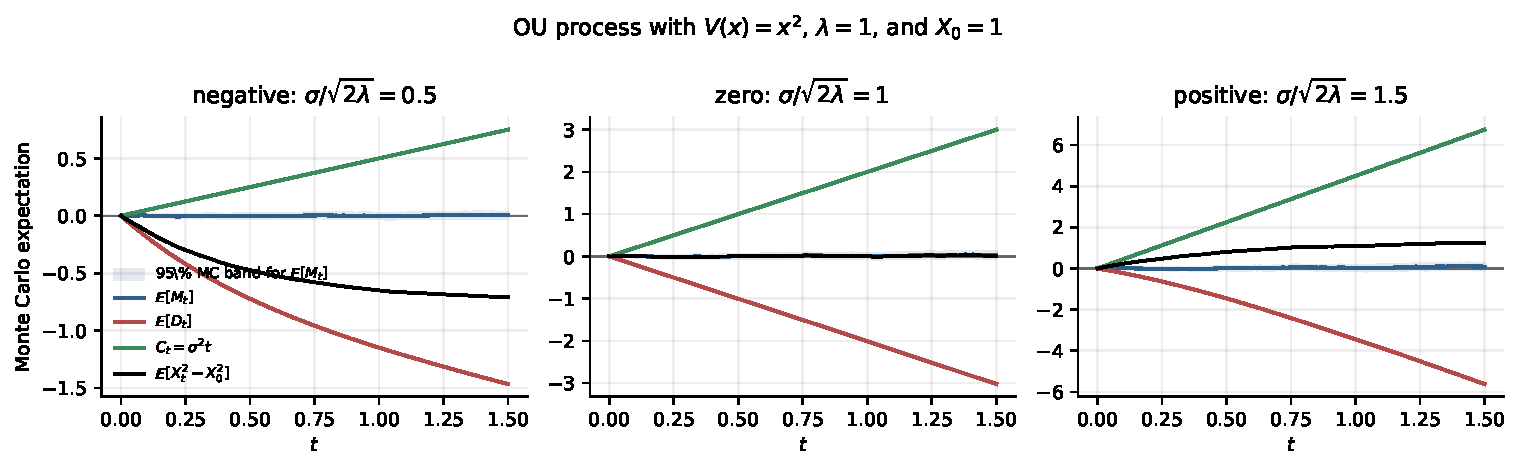
\includegraphics[width=\textwidth]{../log/figures/ou_generator_three_cases.pdf}
  \caption{Monte Carlo expectations from $8000$ Ornstein--Uhlenbeck paths for
  $V(x)=x^2$. The three columns use
  $\sigma/\sqrt{2\lambda}=0.5,1,1.5$. The shaded region is a pointwise
  approximate 95\% Monte Carlo band for $\mathbb E[M_t]$.}
  \label{fig:ou-terms}
\end{figure}

\subsection{Failure of piecewise linearity and success of curvature}

For $f=1$ and $g=\sqrt{2}$ on $[0,1]$, consider a case where want to find a certificate $V$ such that $V(0) = 0$ and $V(1) = 1$.

% the increasing linear candidate
% $V_{\mathrm{PL}}(x)=x$ has
% \[
%   \mathcal{L}V_{\mathrm{PL}}(x)=1>0.
% \]
% More generally, an increasing piecewise-linear certificate must have positive
% slope on some open interval; on that interval its curvature vanishes and
% $\mathcal{L}V=V'>0$. 

A smooth candidate could be:
\[
  V_{\mathcal C^2}(x)=x-\frac{x^2}{2},
\]
the curvature contribution compensates for the positive drift:
\[
  \mathcal{L}V_{\mathcal C^2}(x)
  =(1-x)+\frac12(-1)(2)=-x\leq0.
\]

and indeed $V_{\mathcal C^2}$ is a valid supermartingale certificate.

On the other hand, let's assume $V$ is piecewise linear. 
Then there exists an interval $(x_i, x_{i+1}) \subset [0,1]$ where $V'(x) = a_i > 0$. On that interval, given an $x \in (x_i, x_{i+1})$, the curvature term vanishes, and the generator is
\[
  \mathcal{L}V(x) = V'(x) f(x) + \frac{1}{2} V''(x) g^2(x) = V'(x) f(x) = V'(x) = a_i > 0.
\]

This example motivates the following hypothesis, which we will study in more detail in \autoref{sec:piecewise-quadratic}.

\begin{hypothesis}
  While piecewise linear certificates $V_{\mathrm{PL}}$ are not sufficient to guarantee that $V_{\mathrm{PL}}$ is a supermartingale, \textbf{piecewise quadratic certificates} are sufficient, as the curvature term can compensate for positive drift.
\end{hypothesis}

\begin{figure}[htbp]
  \centering
  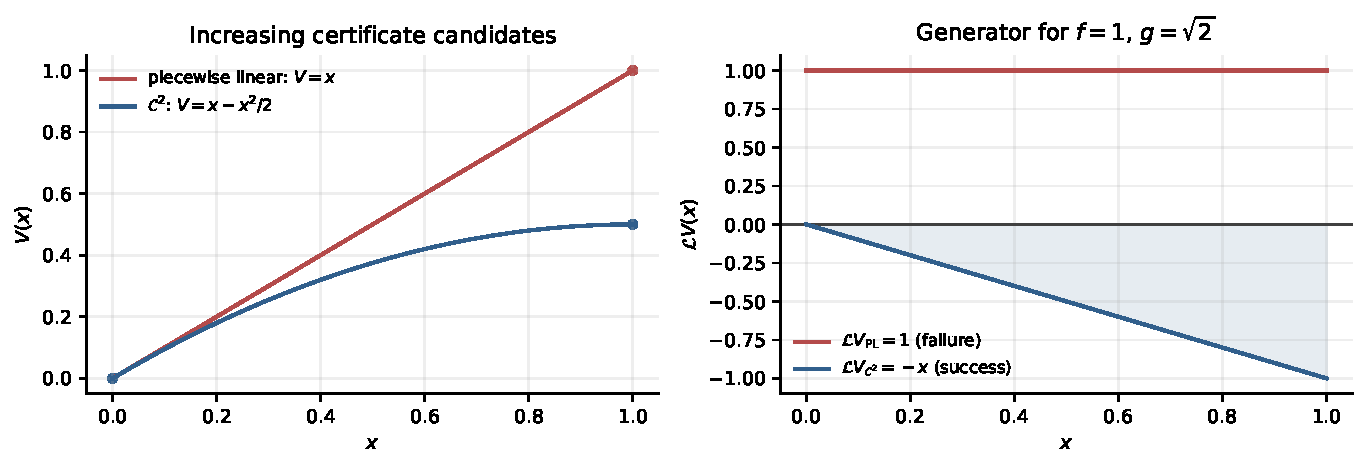
\includegraphics[width=\textwidth]{../log/figures/linear_failure_curvature_success.pdf}
  \caption{An increasing piecewise-linear candidate fails the generator
  condition for $f=1$, $g=\sqrt{2}$, whereas negative curvature makes the
  smooth candidate satisfy it throughout $[0,1]$.}
  \label{fig:linear-vs-curved}
\end{figure}



\subsection{A piecewise $\mathcal{C}^2$ certificate with curvature and a kink}

Finally, let $dX_t=dW_t$ and
\[
  V(x)=
  \begin{cases}
    -\frac12x^2, & x<0,\\
    -x, & x\geq0.
  \end{cases}
\]
Here $D_t=0$, while
\[
  M_t=\int_0^t V'(X_s)\,dW_s,
  \qquad
  C_t=-\frac12\int_0^t\mathbf{1}_{\{X_s<0\}}\,ds,
  \qquad
  K_t=-\frac12L_t^0(X).
\]
Thus $C_t$ decreases while the path lies below zero, and $K_t$ decreases only
when local time accumulates at the kink. Figure~\ref{fig:hybrid-terms} shows
these different mechanisms on the same Brownian realization. The plotted
local time uses an occupation-density approximation with bandwidth $0.06$.

\begin{figure}[htbp]
  \centering
  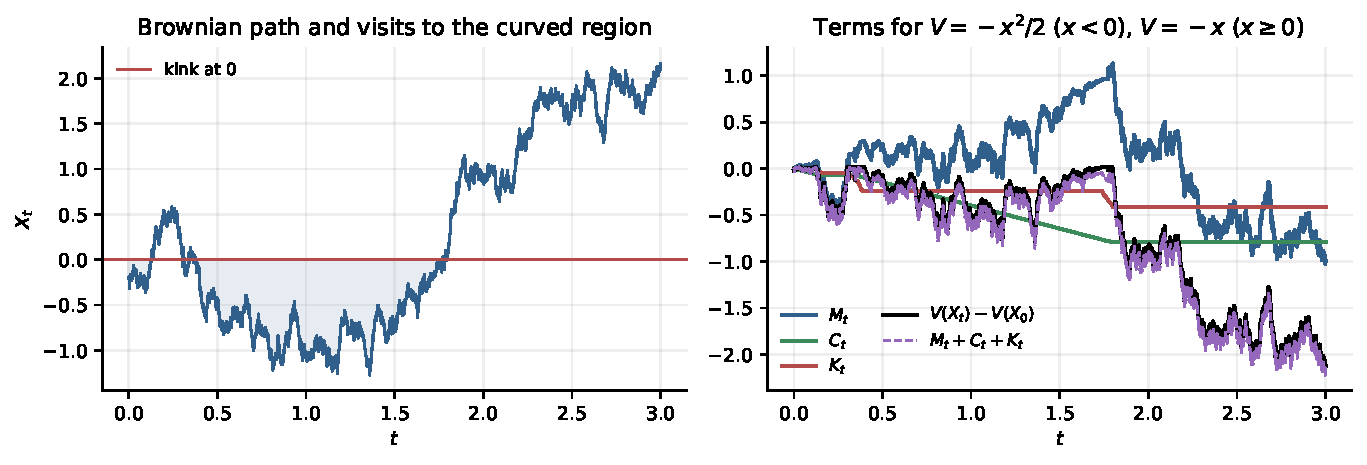
\includegraphics[width=\textwidth]{../log/figures/hybrid_piecewise_c2_terms.pdf}
  \caption{A Brownian realization and the terms for the hybrid piecewise
  $\mathcal C^2$ certificate. The curvature and kink terms are both
  nonincreasing, while the martingale term fluctuates.}
  \label{fig:hybrid-terms}
\end{figure}

\newpage

\section{Piecewise quadratic certificates in dimension one}
\label{sec:piecewise-quadratic}



% \section*{Appendix}

% \subsection*{One dimensional SDEs}

% \subsubsection*{}


\end{document}
